\titre{"glob"} : 
\begin{itemize}
	\item le "$^*$" pour dire toutes les suites de caractères
	\item le "?" pour dire un unique caractère
	\item le "" pour dire a ou b ou c
\end{itemize}

\titre{Expressions régulières POSIX :} Il en existe deux types : basiques et étendues.
\begin{itemize}
	\item le "." pour dire n'importe quel caractère sauf le saut de ligne $\backslash$ n
	\item "car" pour le caractère car
	\item abc pour un a ou b ou c
	\item  pour tout caractère sauf a, b, c
	\item "$\ldots \| \ldots$"
	\item "m$^*$", "m+", "m\{k,l\}
	\item chapeau ou \$
	\item \ldots
	\item Ce n'est pas du tout minimaliste
\end{itemize}

\titre{Expressions régulières à la Kleene :} Les expressions régulières sont données par la grammaire suivante : \\
	$$ ER ::= 0 | 1 | a | ER + ER | ER.ER | ER^* ( 0 = \vide, 1 = \{ "" \}, a = \mathrm{symbole}$$
Les symboles appartiennent ) un ensemble fini appelé alphabet généralement noté $\Sigma$.

\titre{Exemple :} Avec $\Sigma = \{ a, b \}$ :
\begin{itemize}
	\item $0$
	\item $1$
	\item $a$
	\item $b$
	\item $((a+1)^*.b^*)^*+a.b$
\end{itemize}

\titre{Priorités :} $^*$ puis . puis + \\
L'addition est associative et commutative, la concaténation est associative. Le "." est souvent omis.

\titre{Rq :} $r^* = 1 + rr^*$

\titre{Rq :} Deux expressions régulières sont égales si elles correspondent aux mêmes chaines de caractères.

\titre{Langage associé} : On associe à chaque regex $r$ un ensemble de mots sur $\Sigma$ appelé $L(r)$

\titre{Exemples}
\begin{itemize}
	\item $L(0) = \vide$
	\item $L(1) = \{ \varepsilon \}$
	\item $L(a) = \{ a \}$
	\item $L(r_1 + r_2) = L(r_1)\bigcup L(r_2)$
	\item $L(r_1r_2) = \{ mn, m \in L(r_1), n \in L(r_2) \}$ = $L(r_1) . L(r_2)$
	\item $L(r^*) = \{ uu \ldots u, u \in L(r) \}$
	\item $L(0^*) = \{ \varepsilon \}$
	\item $L(1^*) = \{ \varepsilon \}$
\end{itemize}

\titre{Définition :} Un langage $l$ est régulier si il existe une expression régulière $r$ tel que $l=L(r)$
\titre{Regex équivalentes} : Deux expressions sont équivalentes quand elles ont le même langage associé. \\
Question : Peut on vérifier si 2 expressions sont égales ? \\
Question : Existe-t-il des langages non réguliers ? OUI \\
Question : Le complémentaire d'un ensemble régulier est-il régulier ? \\
Question : Peut on tester rapidement si $u\in L(r)$ ? \\
Question : Quand a-t-on $\varepsilon \in L(E)$ ? réponse : on fait une fonction récursive à partir des cas de base : 
\begin{itemize}
	\item $\varepsilon \not\in L(0)$\\
	\item $\varepsilon \in L(1)$\\
	\item $\varepsilon \not\in L(s)$\\
	\item $\varepsilon \in L(E_1 + E_2) \equi \varepsilon \in L(E_1) \ou L(E_2)$
	\item $\varepsilon \in L(E_1E_2) \equi \varepsilon \in L(E_1) \et L(E_2)$
	\item $\varepsilon \in L(E^*)$
\end{itemize}

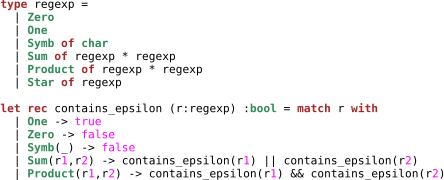
\includegraphics[width=300px]{Images/fig1.pdf}

\titre{Test d'appartenance d'un mot quelconque à $L(R)$ :} \\
On définit $R/a$ la dérivée de $R$ le long de $a$ (première lettre du mot) dont le langage vérifie : 
$$ w \in L(R/a) \equiv aw \in L(R)$$. \\
Pour tester si $w \in L(R)$ : 
\begin{itemize}
	\item Si $w=\varepsilon$ on utilise la méthode vue précédemment
	\item Si $w = aw'$ on vérifie récursivement si $w'\in L(R/a)$
\end{itemize}

\titre{Regles de calcul de $R/a$}
\begin{itemize}
	\item $L(0/a) = L(0)$
	\item $L(1/a) = L(0)$
	\item $L(b/a) = \left\{ \begin{array}{ll} 0 & \mathrm{si} \; b\neq a \\ 1 & \mathrm{si} \; b = a \end{array} \right.$
	\item $L((R_1+R_2)/a) = L(R_1/a + R_2/a)$ 
	\item $L((R_1R_2)/a) = \left\{ \begin{array}{ll} L((R_1/a)R_2 + R_2/a) & \mathrm{si} \; \varepsilon \in L(R_1) \\ L((R_1/a)R_2) & \mathrm{sinon} \end{array} \right.$
	\item $L(R^*/a) = L((R/a)R^*)$
\end{itemize}

A partir de ça on peut programmer l'appartenance d'un mot quelconque au langage d'une expression régulière quelconque. On dit qu'il y a une procédure effective pour le problème "appartenance d'un mot à un langage d'une regex".\\

\titre{Apparté : Montrons que le problème de l'arrêt d'un programme p avec un argument a n'a pas de solution effective. : } On le démontre par l'absurde \\
Supposons qu'un programme résoud ce problème : termine(p,a) renvoie true si p(a) termine, false sinon. \\
On définit un programme oups(x) qui fait la chose suivante :\\
if termine(x,x) (boucle infinie)\\
else return true\\
Quelle est la valeur de oups(oups) ??? Il se termine si il ne se termine pas, sinon il se termine. \\

\titre{Conséquence :} Il n'y a pas de regex dont le langage est exactement l'ensemble des programmes qui terminent.\\

